\documentclass[10pt,a4paper]{article}
\usepackage[utf8]{inputenc}
\usepackage[slovak]{babel}
\usepackage[IL2]{fontenc}
\usepackage{amsmath}
\usepackage{amsfonts}
\usepackage{amssymb}
\usepackage{graphicx}
\usepackage{hyperref}
\usepackage{listings}
\usepackage{ dsfont }
\usepackage{subcaption}
\usepackage{float}
\usepackage[left=2cm,right=2cm,top=2cm,bottom=2cm]{geometry}
\author{Vladimír Macko}
\begin{document}

\pagenumbering{arabic}

\begin{center}
\textbf{Domáca úloha DN2 - WGAN pre text} \\
Vladimír Macko
\end{center}
\medskip

\section{Úloha}
Úlohou bolo zreprodukovať výsledky článku \href{https://arxiv.org/pdf/1704.00028.pdf}{https://arxiv.org/pdf/1704.00028.pdf}. 

Článok pojednáva o novej metóde trénovania architektúry GAN, 
ktorá sa snaží optimalizovať earth mover distance, respektíve Wassersteinovu vzdialenosť.

Optimalizácia tejto vzdialenosti si ale vyžaduje, aby diskriminátor spĺňal Lipschitz constraint a teda aby sa dal vyjadriť ako $1$-Lipšicovská funkcia. 
$1$-Lipšicovská funkcia znamená, že má všade gradienty s normou maximálne 1. 

V pôvodnom článku sa tento problém riešil pomocou "odstrihávania váh" (weight clipping), kde sa v každom kole váhy prenormovali tak, aby mali normu $1$.

Prínosom tohoto článku je, že navrhol optimalizovať funkciu ktorá závisela nie len od Wassersteinovej vzdialenosti ale aj od veľkosti gradientu. Toto sa pre implementáciu ukázalo ako relatívne problematické.

\section{Riešenie}

Autori v článku uvádzajú aj repozitár s ich kódom \href{https://github.com/igul222/improved\_wgan\_training}{https://github.com/igul222/improved\_wgan\_training} ktorý som si forkol do \href{https://github.com/vlejd/improved\_wgan\_training}{https://github.com/vlejd/improved\_wgan\_training}. 
Tento kód je napísaný v pythone a používa knižnicu tensorflow.
Tento kód podľa mňa písal človek, ktorý mal s pythonom (slušným, neakagemickým) veľmi málo skúseností. 
Veľmi ťažkopádne sa používal a obsahoval množstvo zlých programátorských praktík.

Za všetky spomeniem keď auto použil:
\begin{lstlisting}[language=Python]
_iter = [0]
def tick():
	_iter[0] += 1
\end{lstlisting}

Namiesto:
\begin{lstlisting}[language=Python]
_iter = 0
def tick():
	global _iter
	_iter += 1
\end{lstlisting}

Pochopiteľnosť kódu tiež sťažoval tensorflow (a hlavne moja neznalosť tejto knižnice). V kóde sa totiž používa veľké množstvo konvolúcií, ktoré si vyžadujú reshapovanie a permutovanie dimenzii tenzora s ktorým sa počíta.

Cieľ bol teda jasný, prepísať tento kód do knižnice keras (s ktorou mám tiež zatiaľ len veľmi málo skúseností). 

\section{Architektúra}
Opíšme si ale najprv poriadne architektúru ktorú autori použili (z článku som ju mal problém vyčítať). 
Autor ako vstupný text používal prvých 32 (fixná dĺžka + padding) znakov z viet z datasetu Billion words od Googlu. 
Autori nepoužili žiadne predspracovanie. Dokonca v texte nechali všetky nealfanumericke znaky, ktorých sa v pôvodnom datasete nachádza celkom dosť. Predikcie generátora sú potom veľmi dlho počas trénovania "znečistené" týmito znakmi, často na zlých miestach.

Teraz si popíšeme presnú architektúru generátora a diskriminátora. 
Väčšina ďalej spomenutých tenzorov má rozmer $[batch\_size \time 32 \times dim]$, kde $dim$ je dimenzionalita modelu (vo všetkých tenzoroch rovnaká).
Generátor aj diskriminátor pozostávajú z takzvaných reziduálnych blokov (resblock, pozor na zmenu s na z). 
To resblocku príde vstup, na tento input sa dva krát aplikuje relu aktivačná funkcia a 1D konvolúcia veľkosti $5$. 
Tento výstup sa následne prenásobí $0.3$ a priráta k pôvodnému vstupu.
Takéto bloky sa potom ukladajú za seba.

Generátor Najprv vyrobí $128$ rozmerný náhodný vektor. Naň aplikuje "hustú" vrstvu a dostane vektor s rozmermi $[sample\_size \times 32*dim]$, 
ktorý následne pretvaruje do $[batch\_size \times 32 \times dim]$. 
Následne sa $5$ krát aplikuje resblock. Prekvapilo ma že sa nepoužíva žiaden maxpooling.
Posledným krokom je konvolúcia (z $dim$ do $128$ rozmerov, dĺžka konvolúcie je $1$) a softmax, ktoré vyrobia one hot kódovanie generovanej vety.

Diskriminátor vyzerá takmer ako obrátený generátor. 
Najprv konvolúcia z $128$ do $dim$, následne päť krát aplikovaný resblock, a posledná je "hustá" vrstva ktorá robí finálne predikcie. 

Tieto dve časti sa mi aj podarilo prepísať do kerasu. Problém bol, ako prepísať "cost function". 
Problém bol hlavne s gradientovou penaltou.
Nevedel som totiž, ako a či sa môžem v kerase odvolať na gradiente pri rátaní chyby a ako správne upraviť kerasový pipeline aby to podporoval. 
Som si istý, že to ide, ale v momente ako som to zistil som sa rozhodol radšej upraviť pôvodný kód a skúsiť ho na iných dátach.

Autor pri rátaní gradientu postupoval nasledovne. 
Zobral reálne dáta $\mathrm{rd}$ a vygenerované dáta $\mathrm{fd}$ a zrátal bod pre rátanie gradientu ako $\mathrm{gd}= \mathrm{rd}(1-\alpha) + \mathrm{fd}\alpha$, kde $\alpha$ je nahodný vektor rozmerov $[batch\_size \times 1 \times 1]$, a teda pre každý vstup sa náhodne rozhodol ako veľmi je reálny a ako veľmi je z generátora.
Následne zistil gradient diskriminátora v bode $\mathrm{gd}$ a pridal ho do chybovej funkcie.

Ako optimalizátor použil Adama s rýchlosťou učenia $1e-4$, $\beta_1=0.5$ a $\beta_2=0.9$.

Následné trénovanie fungovalo tak, že v každej epoche sme sa generátorom vygenerovalo niekoľko príkladov, niekoľko prikladov sa vybralo z reálnych dát, na týchto dátach sa po dobu niekoľkých epôch ($20$) trénoval diskriminátor. Následne sa urobil update generátora.

\section{Chybové funkcie}

Autor priebežne rátal (vykresľoval a ukladal) chybu diskriminátora. 

$$L = \underset{\tilde{x} \sim \mathds{P}_g }{\mathds{E}} [D(\tilde{x})] - \underset{\tilde{x} \sim \mathds{P}_r }{\mathds{E}}[D(\tilde{x})] + \lambda\underset{\hat{x} \sim \mathds{P}_{\hat{x}}}{\mathds{E}} [(\parallel \nabla_{\hat{x}}D(\hat{x}) \parallel_2 - 1)^2]$$

Okrem toho pribežne pozoroval kvalitu generátora. 
Na pôvodných dátach natrénoval $1$-gram, $2$-gram, $3$-gram a $4$-gram jazykový model. 

Následne natrénoval takéto $n$=gramové modely aj na generovaných dátach a zaznamenával Jensen–Shannonovu vzdialenosť od tých trénovaných na reálnych.


\section{Experimenty}

Kvôli týmto experimentom som musel obetovať svoju zásobu mrazenej zeleniny a plechovkového piva, ktoré som počas experimentov musel mať položené na notebooku, aby sa mi kvôli náročným výpočtom a veľkému teplu neprehrial.


\subsection{Billion words}

Ako prvé som sa pokúsil zreprodukovať výsledky z článku (priečinok cuted). Z časových dôvodov a výpočtových dôvodov som ale musel použiť len časť Billion words datasetu, konkrétne prvých $1000000$. Taktiež som nemohol použiť veľkosť dimenzie $500$, ako bolo použité v článku, ale len maximálne $300$. 
Trénoval som po dobu $1300$ epôch. V článku nie je úplne jasné, koľko epôch použili autori.

Tu sú ukážky textu z článku
\begin{verbatim}
Busino game camperate spent odea
In during the Uitational questio       
Dour Fraps higs it was these del
Divos from The ’ noth ronkies of
\end{verbatim}

Vidíme, že tieto texty vyzerajú na prvý pohľad ako normálny jazyk. 
Sú použité rozumné písmená, rozumne sa striedajú samohlásky a spoluhlásky, veľké písmená sú na začiatkoch slov.
Dáta ale stále obsahujú nezmyselné slová.

Pre porovnanie, takto vyzerajú reálne dáta.
\begin{verbatim}
Brent North Sea crude for Novemb
That seems to have been their mo
Gordon will join Luol Deng on th
Nikam maintains the attacks were
\end{verbatim}

Name natrénovaný model mal nasledovné výsledky:
\begin{verbatim}
" Is outhis Darners ame e8 ) mat
Uo‚ wuaut twen ist whit worl th
Thr werk  It a Powast wo tdepe 
\end{verbatim}

Upozorňujem, že naše dáta neboli cherry pickované. Vidíme, že ich kvalita je o čosi horšia, no dáta majú isté kvality. 
Správne používanie veľkých písmen, rozumný pomer písmen, správne medzery.

\begin{figure}[H]
    \centering
    \begin{subfigure}[b]{0.4\textwidth}
        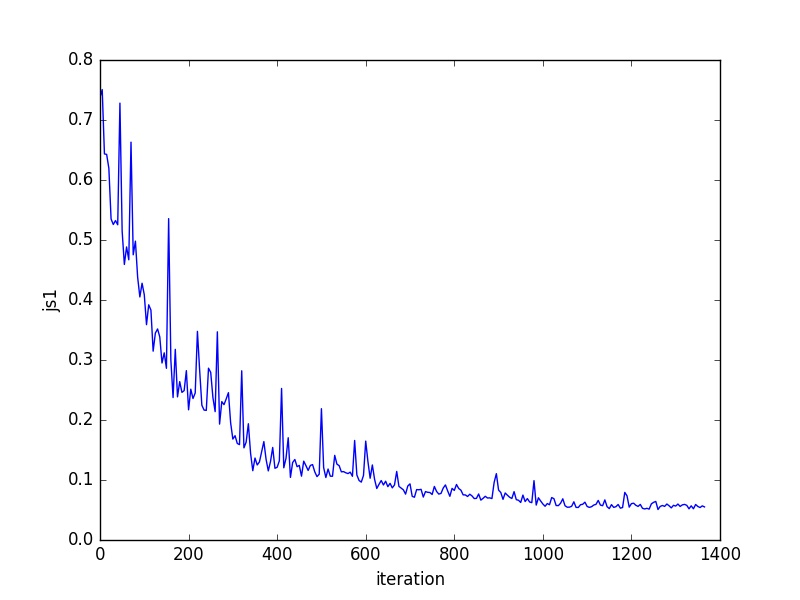
\includegraphics[width=\textwidth]{cuted/js1}
        \caption{$1$-gram}
    \end{subfigure}
    ~ 
    \begin{subfigure}[b]{0.4\textwidth}
        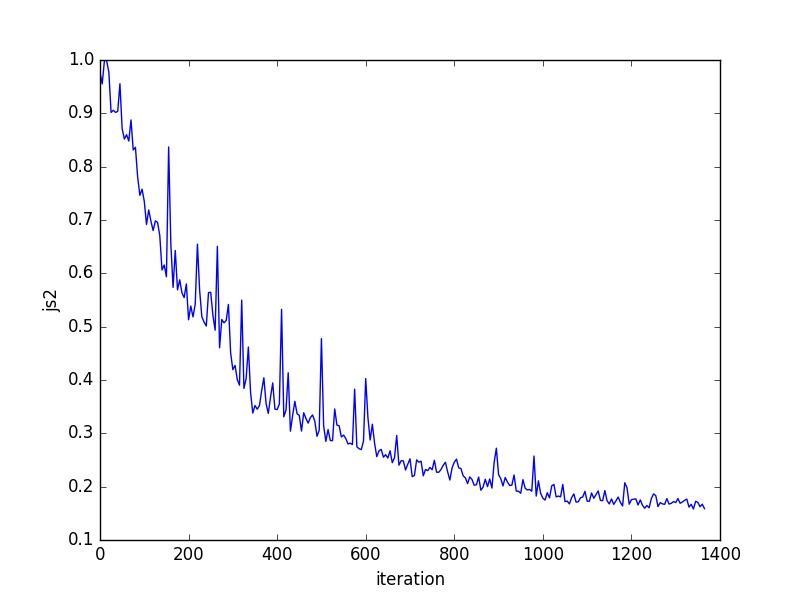
\includegraphics[width=\textwidth]{cuted/js2}
        \caption{$2$-gram}
    \end{subfigure}
    
    \begin{subfigure}[b]{0.4\textwidth}
        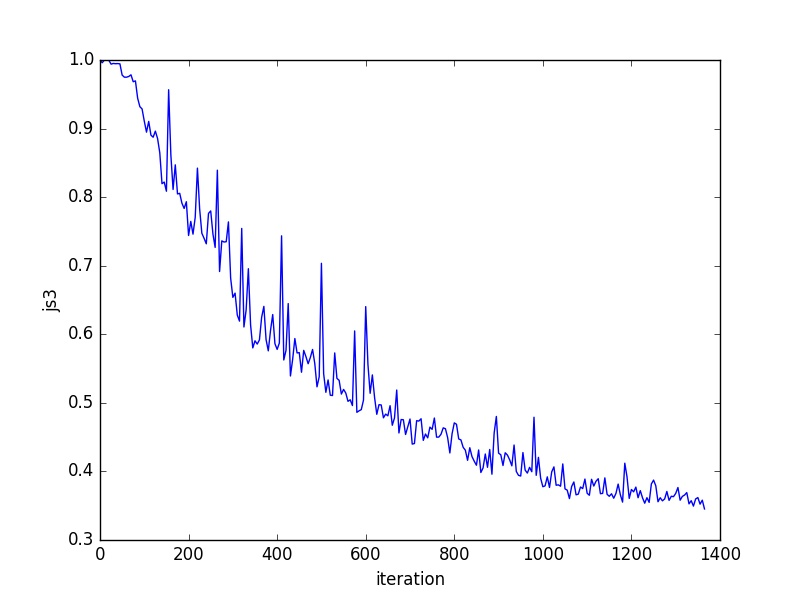
\includegraphics[width=\textwidth]{cuted/js3}
        \caption{$3$-gram}
    \end{subfigure}
    ~ 
    \begin{subfigure}[b]{0.4\textwidth}
        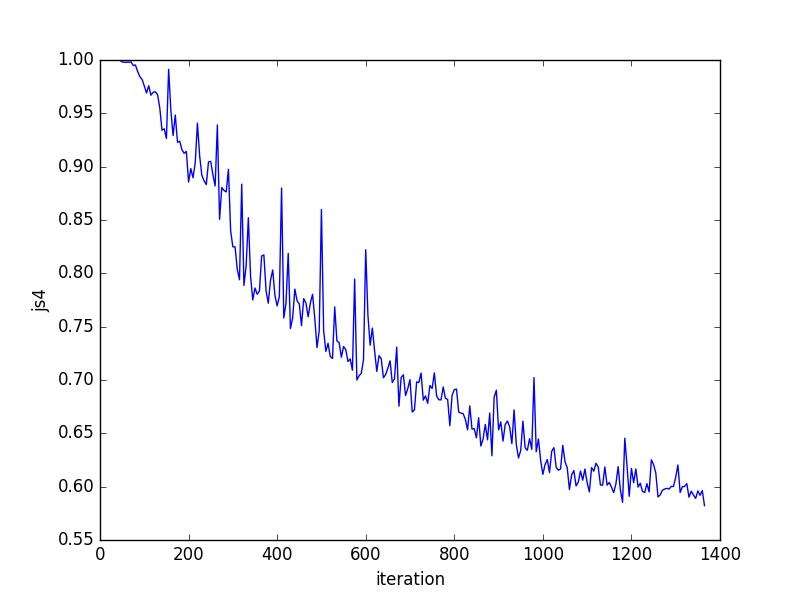
\includegraphics[width=\textwidth]{cuted/js4}
        \caption{$4$-gram}
    \end{subfigure}
    \caption{JS divergencia oproti $n$-gramom (billion words)}\label{fig:animals}
\end{figure}
\begin{figure}[H]
	\centering
	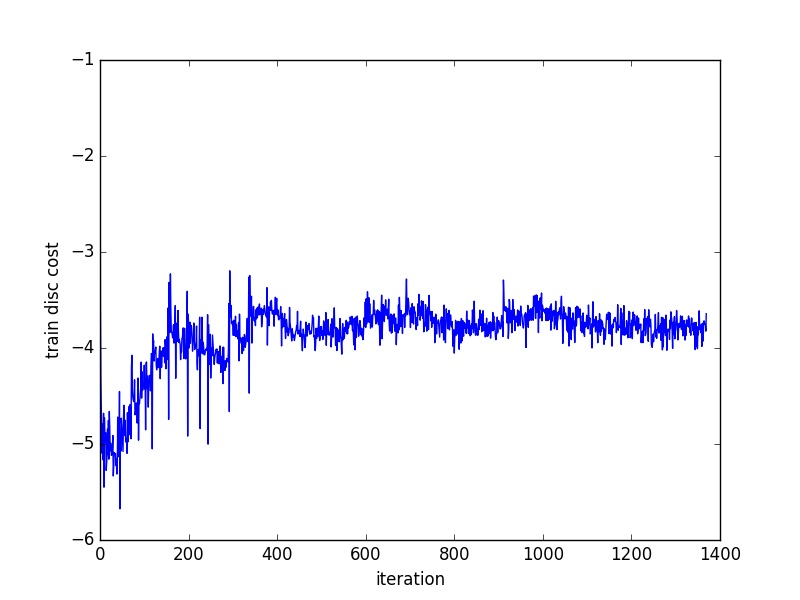
\includegraphics[width=0.5\textwidth]{cuted/train_disc_cost}
    \caption{Chyba diskriminátora (billion words) }
\end{figure}

Zaujímavé je, že v našom prípade sa síce ešte generátor zlepšoval (v porovnaní s $n$-gramovým modelom), ale chyba diskriminátora už veľmi (takmer vôbec) nerástla. 

Ako druhý experiment sme skúsili použiť ten istý dataset, ale s dimenziou modelu len $200$ (priečinok cuted\_small).

Na prvý pohľad vyzerajú dáta ešte o trochu lepšie (keď sa podarí). Zaujímavé je, že v chybách medzi týmto modelom a tým s dimenziou $300$ nie je vôbec veľký rozdiel, aj keď bol tento model trénovaný o trochu menej epôch ($1000$). 
\begin{verbatim}
Dtrinnges tonto as gig cand in n
Comesnimiog tnk oo reos tho Dtna
A Shin nohe fom tennne han enid 
The rospin Site A fter erthe Ant
\end{verbatim}



\begin{figure}[H]
    \centering
    \begin{subfigure}[b]{0.4\textwidth}
        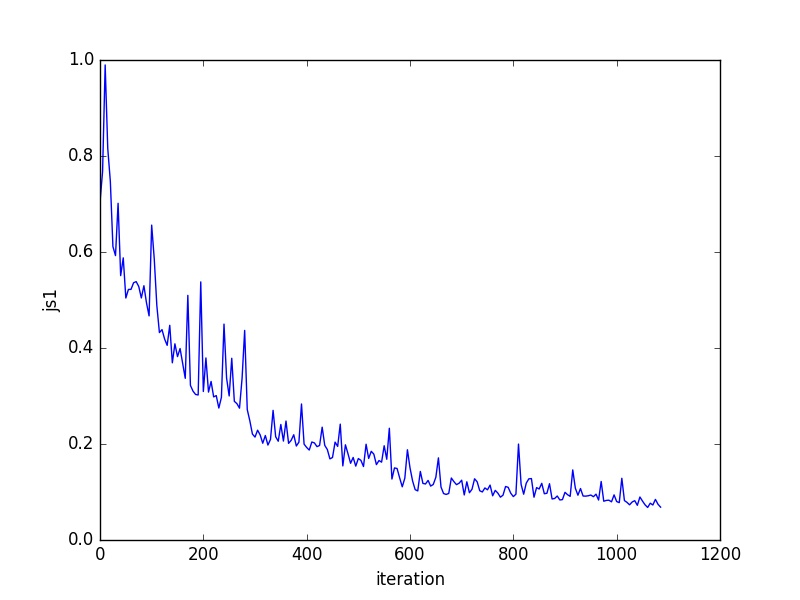
\includegraphics[width=\textwidth]{cuted_small/js1}
        \caption{$1$-gram}
    \end{subfigure}
    ~ 
    \begin{subfigure}[b]{0.4\textwidth}
        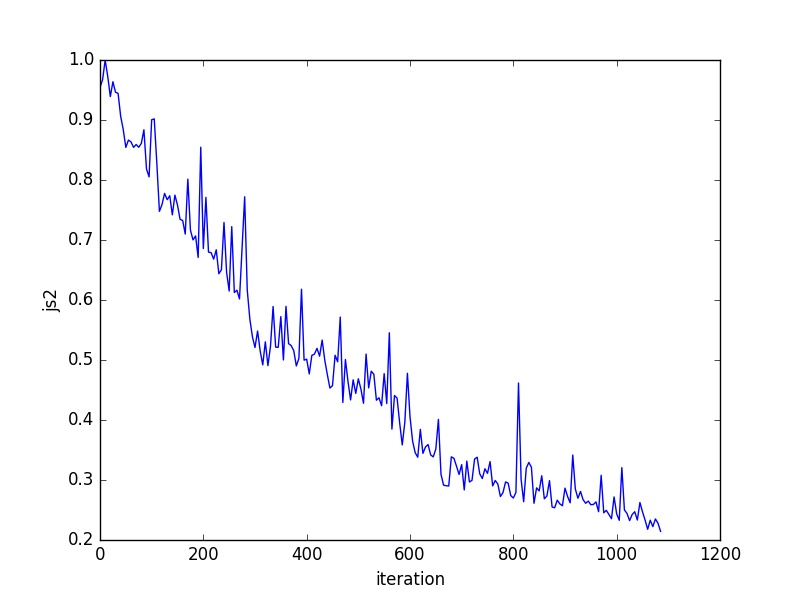
\includegraphics[width=\textwidth]{cuted_small/js2}
        \caption{$2$-gram}
    \end{subfigure}
    
    \begin{subfigure}[b]{0.4\textwidth}
        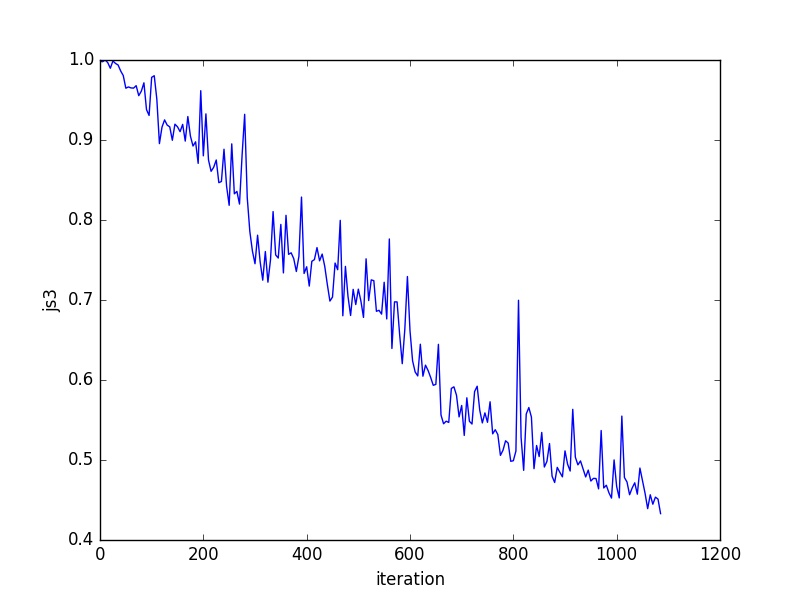
\includegraphics[width=\textwidth]{cuted_small/js3}
        \caption{$3$-gram}
    \end{subfigure}
    ~ 
    \begin{subfigure}[b]{0.4\textwidth}
        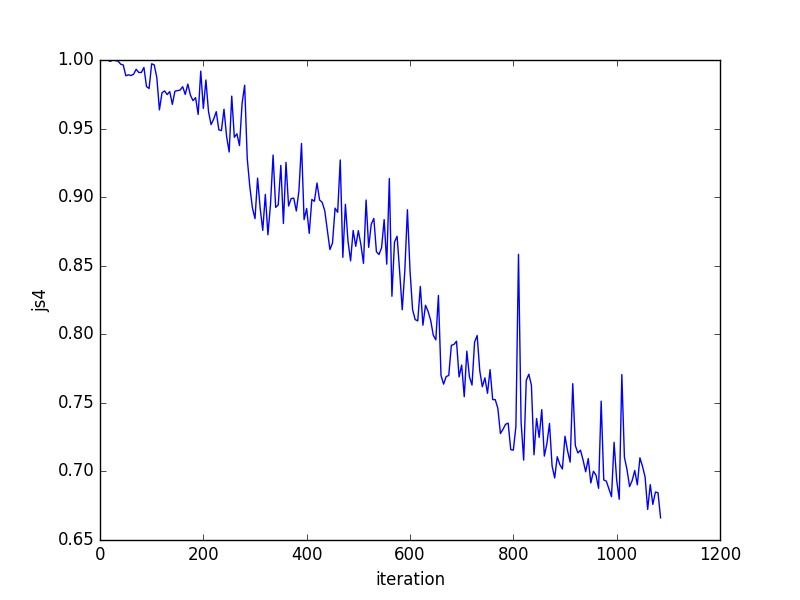
\includegraphics[width=\textwidth]{cuted_small/js4}
        \caption{$4$-gram}
    \end{subfigure}
    \caption{JS divergencia oproti $n$-gramom (billion words 200)}\label{fig:animals}
\end{figure}
\begin{figure}[H]
	\centering
	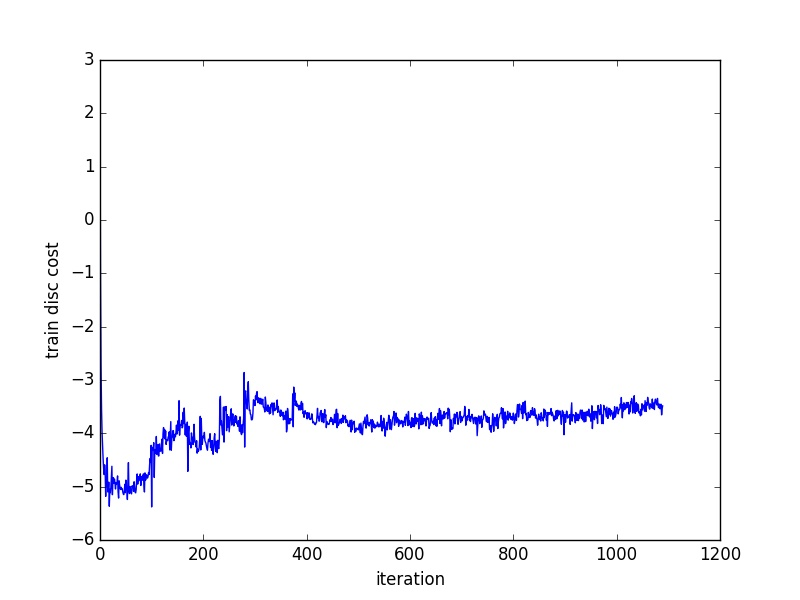
\includegraphics[width=0.5\textwidth]{cuted_small/train_disc_cost}
    \caption{Chyba diskriminátora (billion words 200) }
\end{figure}

\subsection{Shakespeare}
Ako ďalší sme použili oveľa menší dataset a to Shakespearove hry. 
Dáta sme získali pomocou knižnice nltk, kde je to (takmer) štandardný korpus.
Tieto dáta sme pozmenili tak, aby každý riadok začínal veľmi podobne. 
Ospravedlňujem sa za chybu v slove speech, všimol som si to až teraz.

Príklad dát:
\begin{verbatim}
Speach 1: That I have much ado t
Speach 2: Your mind is tossing o
Speach 2: There, where your argo
Speach 2: Like signiors and rich
\end{verbatim}


Náš model po $85$ epochách:
\begin{verbatim}
Speach tt te ah eh h htah ec aah
Speach hh  tah  eh ahaeh eeaahh 
Speach ee  eh et ach eth  ht  h 
Speacthc etc  e  tt hee ah  ah  
\end{verbatim}

Náš model po $200$ epochách:
\begin{verbatim}
Speach 3q3 ahte 3hpe Speach tatt
Speach 3c3 ppa3  s6t  ath ee at 
Speach asacp e 3hce3th e  sath a
Speach l3 thpba3 s sa 6s3a te ah
\end{verbatim}

Náš model po $600$ epochách:
\begin{verbatim}
Speach 3: Inothdthee o pas And f
Speach 1h: parlaielmfca fsherth 
Speach 2: Thaneat si thf theu m 
Speach 23: Sheal h ueald hand ih
\end{verbatim}

Je krásne vidno ako si model postupne začal uvedomovať, čo musí byť na začiatku riadku.

\begin{figure}[H]
    \centering
    \begin{subfigure}[b]{0.4\textwidth}
        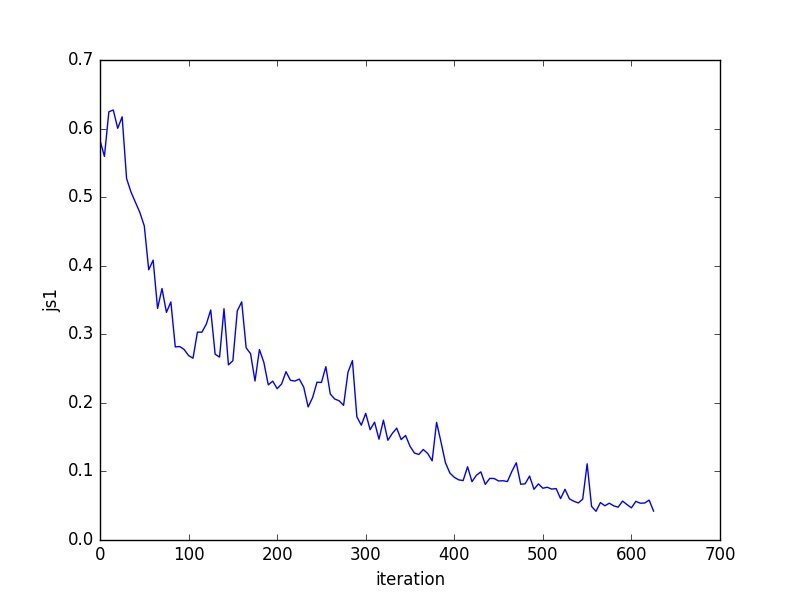
\includegraphics[width=\textwidth]{romeo/js1}
        \caption{$1$-gram}
    \end{subfigure}
    ~ 
    \begin{subfigure}[b]{0.4\textwidth}
        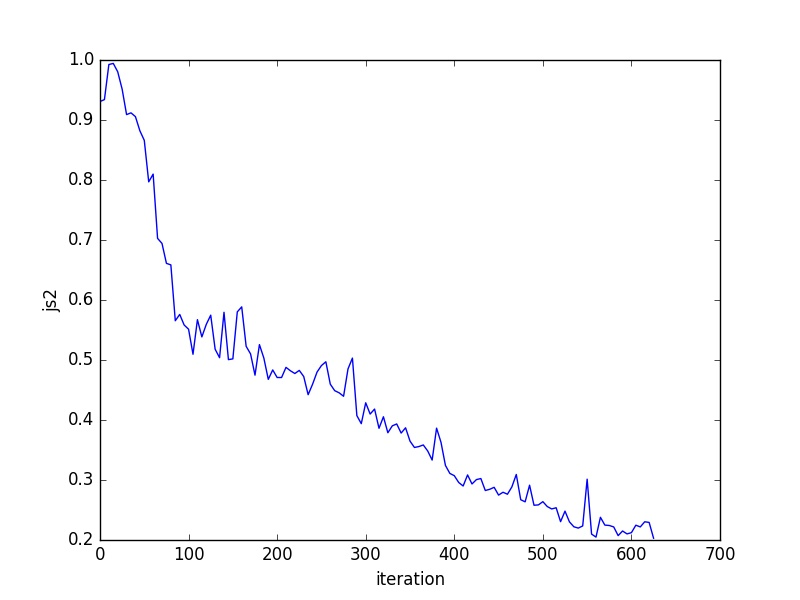
\includegraphics[width=\textwidth]{romeo/js2}
        \caption{$2$-gram}
    \end{subfigure}
    
    \begin{subfigure}[b]{0.4\textwidth}
        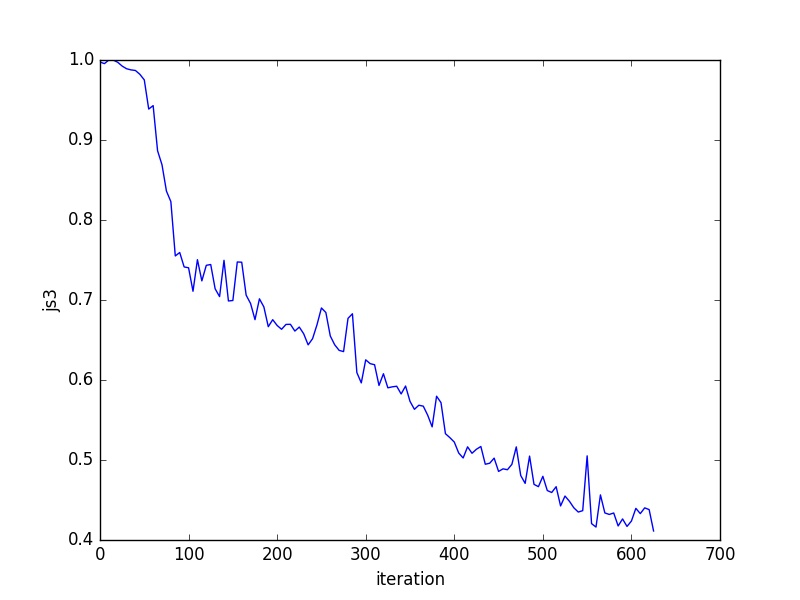
\includegraphics[width=\textwidth]{romeo/js3}
        \caption{$3$-gram}
    \end{subfigure}
    ~ 
    \begin{subfigure}[b]{0.4\textwidth}
        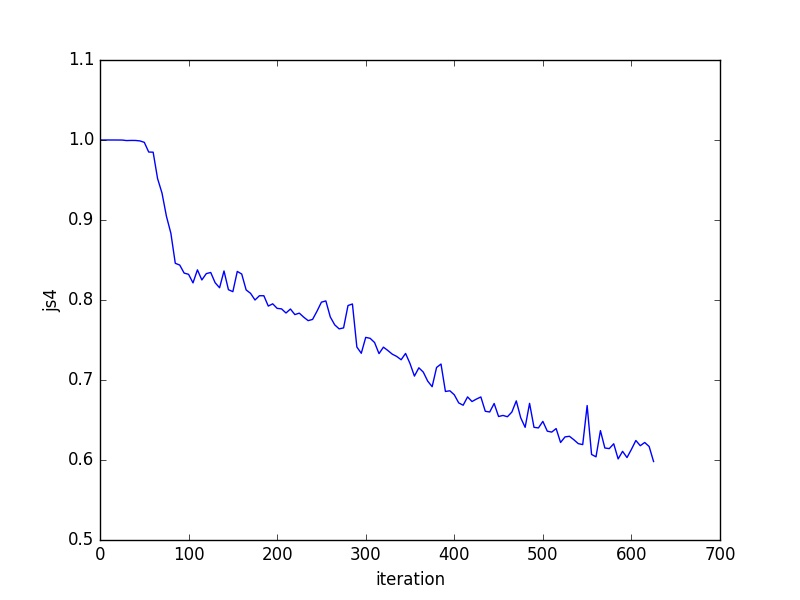
\includegraphics[width=\textwidth]{romeo/js4}
        \caption{$4$-gram}
    \end{subfigure}
    \caption{JS divergencia oproti $n$-gramom (shakespeare)}\label{fig:animals}
\end{figure}
\begin{figure}[H]
	\centering
	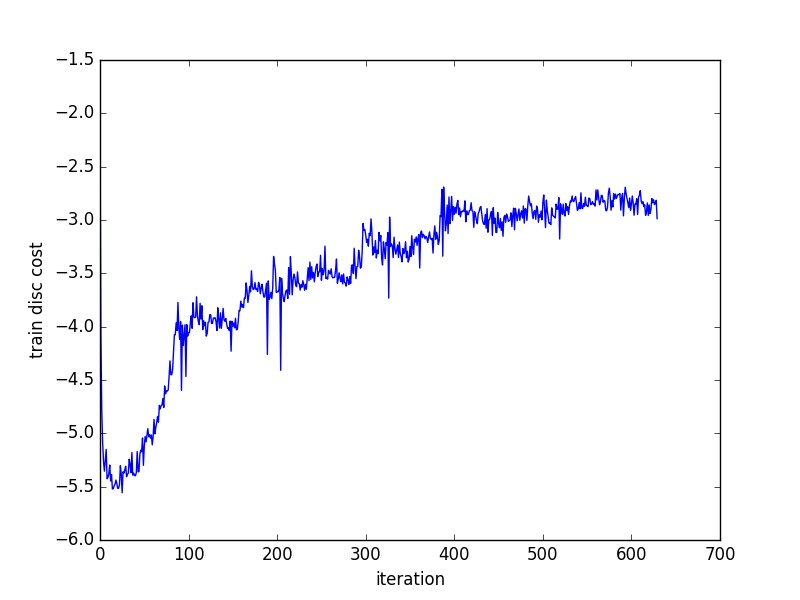
\includegraphics[width=0.5\textwidth]{romeo/train_disc_cost}
    \caption{Chyba diskriminátora (shakespeare) }
\end{figure}


\subsection{Quora}
Ďalší dataset ktorý som skúsil boli otázky z quori. 
Tento dataset je z kagglovej súťaže "Quora question pairs".
Tieto dát boli jemne predspracované, boli lowercasnotú a boli z nich odstránené niektoré nealfanumerické znaky. 

\begin{verbatim}
how does the surface pro himself
should i have a hair transplant 
what but is the best way to send
which food not emulsifiers ?
\end{verbatim}

\begin{verbatim}
what iee he ehe  anw anoi mnoe t
what aho s oan ant ln law rt iro
what is ihe terthent8eetsacfteei
what msmihethinc aren ina miteie
\end{verbatim}


\subsection{Kanye}
Keďže výsledky nášho modelu boli celkom dobré, ale pre potreby bežnej reči ešte nedostatočné, rozhodli sme sa ako posledný dataset použiť texty speváka Kanye West.

Tento dataset mal len $6554$ riadkov a preto dúfame, že na ňom bude mať generátor naozaj dobré výsledky.




\section{PC špecifikácia}
Experimenty som bečal na osobnom notebooku lenovo Y 700, procesor Intel(R) Core(TM) i7-6700HQ CPU @ 2.60GHz, graficka karta GM107M [GeForce GTX 960M] 4GB, 16GB operačná pamäť.

\section{Linky}
Dáta s popisom a zdrojmi: \href{https://drive.google.com/drive/folders/0B7MLuc1jq3A8eFpVWUZ0eDEwdlE?usp=sharing}{https://drive.google.com/drive/folders/0B7MLuc1jq3A8eFpVWUZ0eDEwdlE?usp=sharing}

Môj vyčistený fork: \href{https://github.com/vlejd/improved\_wgan\_training}{https://github.com/vlejd/improved\_wgan\_training}

\end{document}